\documentclass[12pt]{article}

\usepackage{graphicx}
\usepackage{caption}
\usepackage{amsmath, amssymb, amsthm}
\usepackage{booktabs}
\usepackage{enumitem}
\usepackage{geometry}
\geometry{margin=1in}
\usepackage{xcolor}
\usepackage{float}
% \usepackage[numbers,sort&compress]{natbib} % number style
\usepackage[colorlinks=true, allcolors=blue]{hyperref} %For hyperlinks, usually must be the last package called
\usepackage[capitalise]{cleveref} % must be loaded after hyperef
\usepackage{tabularx}
\usepackage{float}



% Packages for algorithms and pseudocode
\usepackage{algorithm}
\usepackage{algpseudocode}

\title{NPSC3000 End of Year Report: Can Reinforcement Learning Outperform Traditional Methods for Cloud Resource Allocation}
\author{
\textbf{Student:} Ty Riekert \\
\textbf{Supervisor:} Elham Mardaneh \\
\textbf{Co-supervisor:} Tony Mathew
}
\date{Sept 2026}



\begin{document}
\maketitle
\begin{abstract}
The problem of resource allocation (RA) is a critical issue amongst cloud providers \cite{saidi2023, sdn2021, vinothina2012, parikh2013, mohamaddiah2014}. A shared set of physical resources -- servers, network, storage -- must be dynamically allocated to jobs arriving in real time, and ensuring operational efficiency, traffic performance, and energy conservation is a vital ongoing challenge. This can be modelled as a resource-constrained scheduling optimisation problem; where jobs arrive dynamically and must be assigned without foreknowledge of the future, the problem is \textit{online}. Since cloud RA is inherently multi-objective and dynamic, traditional methods have been shown to struggle \cite{lbts2024, 10854610, DAHMANI2025100616, hu2021attend2pack}, and recent studies highlight the strong potential of reinforcement learning (RL) in handling dynamic, large-scale environments of this kind \cite{saidi2023, autoscaling2023, lbts2024, dynamic2026}. This report implements and rigorously evaluates RL agents against traditional methods on tardiness, jobs scheduled, and total objective reward, across both an offline (fully-known-in-advance) and an online (dynamic-arrival) formulation of the problem.

Two RL algorithms were implemented and iterated on extensively: proximal policy optimisation (PPO) and advantage actor-critic (A2C). On the raw joint job-and-machine action space, PPO failed to learn deadline-aware scheduling under every configuration tested -- reward tuning, a Lagrangian-constrained variant, a tardiness-focused hyperparameter search, and a pointer-network architecture all converged to tardiness statistically indistinguishable from a heuristic that ignores deadlines entirely. A2C with potential-based reward shaping \cite{ng1999shaping} achieved a genuine, if narrower, win on the fixed-instance setting, but this did not survive training on randomized instances, and a constrained variant (RCPO) that briefly appeared to be the project's best result was later found to be achieving it by abandoning jobs rather than scheduling them well, and did not hold up under a 3-seed rigor check. The resolving change was architectural, not algorithmic: reducing PPO's action space from a joint (job, machine) choice to a smaller, structured decision -- most successfully, having the agent select \emph{which classical dispatching rule} to apply at each tick -- closed almost the entire gap to the proven-optimal floor found by an exact CP-SAT solver, reaching a tardiness of 11.00 against a proven optimum of 8.00 (EDF, the strongest single fixed heuristic, reaches 16.00). This result is best understood as a \emph{selection hyper-heuristic} that has learned when to defer to each of several existing rules, not as RL discovering novel scheduling behaviour from scratch -- a materially different, more modest, but still genuine and citable claim. In the online setting, the same action-space-reduction approach outperforms most heuristics under sustained load, but training for longer consistently regresses performance toward a single dominant rule, a phenomenon confirmed across three independent runs and not yet resolved. Fully closing the remaining gap to the best classical heuristics, and understanding the online case's instability, remain open work.

\end{abstract}


\newpage
\section{Project Deliverables}
The aim of this project is to formulate cloud resource allocation as a mathematical optimisation and reinforcement learning problem, and to implement and rigorously evaluate RL models against established methods. The specific deliverables are:
\begin{itemize}
    \item Conduct comprehensive research on current findings and machine learning in cloud resource allocation
    \item Formulate a mathematical model of the cloud RA problem, expressed as a resource-constrained scheduling optimisation problem
    \item Create a corresponding Markov Decision Process (MDP) formulation of the reinforcement learning agent
    \item Implement the code of the scheduling environment
    \item Implement the code for the reinforcement learning agent(s)
    \item Evaluate the trained agents against classical scheduling heuristics to determine under what conditions reinforcement learning outperforms traditional methods.
\end{itemize}
The last item was not delivered as a single train-and-compare run, but as an iterative process repeated throughout the entire second half of the project: a constant loop of training, evaluating against baselines, examining and researching the behaviours and faults this surfaced, and revising the design accordingly. This iterative cycle -- \emph{benchmark, diagnose, research, revise} -- is itself a deliverable in the sense that it establishes, empirically and with literature grounding, which design choices are load-bearing for scheduling performance and which are not.

\section{Background}
\subsection{Cloud Computing}
Cloud computing refers to the use of computing services and resources delivered over the internet, and resource allocation (RA) is one of the most critical challenges facing cloud providers today \cite{huawei2022, saidi2023}. As cloud infrastructure underpins the majority of modern computing services, effectively allocating physical resources like compute or network bandwidth to a continuously arriving stream of workloads has become of vital importance to providers \cite{sdn2021}. Poor allocation can lead to poor outcomes in response time, environmental sustainability (energy and power efficiency), throughput, makespan, utilisation, and more \cite{cloudkpi2010, dvbpp2026, mohamaddiah2014, anuradha2014}.

\subsubsection{Cloud RA}
Cloud RA can be decomposed into several coupled problems. Virtual machine (VM) placement maps user requests onto a provider's physical servers, virtualised as VMs, subject to resource constraints like CPU and memory; this is widely regarded as the core RA subproblem \cite{saidi2023}. Task scheduling divides the workload evenly across all available resources while minimising execution and response time \cite{lbts2024}. Autoscaling dynamically adjusts resource capacity to match fluctuating demand in real time \cite{autoscaling2023}, and load balancing distributes incoming tasks evenly to avoid hotspots \cite{lb2024}.

Solutions to these formulations generally fall into three categories:
\begin{itemize}
    \item \textbf{Exact Methods}. Algorithms that always solve a problem to provable optimality (e.g. linear/integer programming, constraint programming).
    \item \textbf{Approximation Methods}. Used when exact algorithms become computationally infeasible. Two main classes are heuristics -- algorithms designed to quickly construct or improve a single solution -- and metaheuristics, which are higher-level strategies that guide heuristic search \cite{alkhalifa2025comparative}.
    \item \textbf{Machine learning}. Methods that learn a decision rule directly from data or experience, rather than following a fixed hand-designed procedure.
\end{itemize}
Exact methods guarantee optimality but do not scale past small instances, since RA problems of this kind are typically NP-hard \cite{approx2015}. Heuristics and metaheuristics scale to realistic problem sizes, but cannot guarantee optimality, and their solution quality depends heavily on how well the rule or search procedure happens to fit the specific instance and workload distribution encountered. Systematic reviews within this field identify four recurring limitations of these approximation methods: scalability, adaptability, generalisation, and multi-objective complexity \cite{lbts2024, mohamaddiah2014, ml_ra_litrev2025}.

\subsubsection{Motivations for Machine Learning}
These limitations motivate a growing body of work applying machine learning, and reinforcement learning specifically, to combinatorial and scheduling problems. A fixed heuristic encodes one designer's intuition about which job to prioritise, evaluated once at design time; it cannot adapt when the workload distribution it sees in deployment differs from what its designer anticipated. RL instead learns a policy from interaction with the environment, adapting to whatever distribution of jobs it is trained and evaluated against \cite{ml_ra_litrev2025}. Recent systematic reviews of RL applied to bin-packing and scheduling problems report rapid growth in this area, with a clear shift from simple rule-based tactics toward deep RL techniques in complex, multi-dimensional settings \cite{DAHMANI2025100616}, and RL-based approaches have begun to demonstrate results competitive with classical heuristics on cloud and bin-packing problems specifically \cite{10854610, hu2021attend2pack}. At the same time, the literature identifies real open gaps: dynamic VM placement remains comparatively under-explored by machine learning relative to its static counterpart, and generalisation of a learned policy to workload distributions it was not trained on remains a largely open problem \cite{ml_ra_litrev2025, DAHMANI2025100616}. This project treats "does RL outperform traditional methods here" as an empirical question to be tested rigorously, rather than assumed -- across a fixed instance, a randomized-instance distribution, and a dynamic-arrival online setting -- which is precisely where this report's results turned out to be more nuanced than a simple yes.

\subsection{Reinforcement Learning}
\subsubsection{Markov-Decision Process}
Reinforcement learning problems are formalised as Markov Decision Processes (MDPs), a tuple $(\mathcal{S}, \mathcal{A}, P, R, \gamma)$ of a state space, action space, transition function, reward function, and discount factor \cite{DRL_Intrusion}. At each discrete step $t$, an agent observes a state $s_t \in \mathcal{S}$, selects an action $a_t \in \mathcal{A}$ under a policy $\pi$, and receives a reward $r_t = R(s_t, a_t)$ before transitioning to $s_{t+1}$ according to $P(s_{t+1}\mid s_t, a_t)$. The agent's objective is to find a policy that maximises expected discounted return $\mathbb{E}\left[\sum_t \gamma^t r_t\right]$. The optimal state-value function $V^{*}(s)$ satisfies the Bellman optimality equation,
\begin{equation}
      V^{*}(s) = \max_{a \in \mathcal{A}} \left( R(s,a) + \gamma \sum_{s'
  \in \mathcal{S}} P(s'|s,a)\,V^{*}(s') \right),
\end{equation}
which can in principle be solved exactly by dynamic programming for small, fully enumerable $\mathcal{S}$ and $\mathcal{A}$. For a scheduling problem of this project's scale -- where the state includes every unscheduled job's features and every machine's remaining capacity, and the action space is a choice over job/machine pairs -- $\mathcal{S}$ and $\mathcal{A}$ are far too large to enumerate, motivating a function-approximation approach in which a neural network approximates the policy and/or value function directly, rather than solving the Bellman equation exactly.

\subsubsection{Algorithms}
Policy-gradient methods parameterise the policy $\pi_\theta$ directly and optimise $\theta$ by gradient ascent on expected return, using the policy gradient theorem \cite{sutton2000policy}. Actor-critic methods -- combining a policy (\emph{actor}) with a learned value function (\emph{critic}) used as a variance-reducing baseline -- are the dominant modern family \cite{konda1999actorcritic}, and were selected here because the task has a discrete action space (ruling out continuous-control methods such as DDPG/TD3/SAC) and a long decision horizon that benefits from a learned value baseline over pure REINFORCE-style Monte-Carlo estimation \cite{williams1992reinforce}. Two actor-critic algorithms were implemented and compared:
\begin{itemize}
    \item \textbf{Proximal Policy Optimisation (PPO)} \cite{lehmann2024policygradients} clips the policy-update ratio to a small trust region around the previous policy, giving TRPO-like update stability with first-order optimisation. It is widely used, well-supported by existing libraries, and was the primary algorithm used throughout this project.
    \item \textbf{Advantage Actor-Critic (A2C)} \cite{aigreeksActorCritic, apxml_a2c_a3c_2026} performs a synchronous, on-policy actor-critic update using multiple parallel rollouts. It has no publicly-maintained masked-action implementation in this project's chosen RL library (Stable-Baselines3), so a hand-rolled masked A2C was implemented for this project specifically.
\end{itemize}
Both support discrete, maskable action spaces (required so that infeasible job/machine placements can be excluded from sampling), and both were used throughout this project's experiments, with the specific choice between them depending on the experiment (detailed in Methodology).

\section{Methodology}

\subsection{Problem Formulation}
The offline case considers a cloud computing environment with a set of jobs, each with a fixed processing duration and fixed resource requirements (e.g. CPU, memory), that must be assigned to a set of physical machines. Each job is treated as independent, but is given a priority weight $w_j$ representing an externally-assigned importance (e.g. a service-level-agreement tier, contractual priority, or business criticality) that a downstream operator has already determined -- this project does not model \emph{why} a job has a given weight, only that scheduling should respect it. Machines are restricted only by their own resource capacity, and may hold multiple jobs simultaneously provided their combined resource usage does not exceed that capacity; once assigned, a job remains on its machine until completion (no migration).

\begin{table}[htbp]
\centering
\caption{Nomenclature}
\label{tab:nomenclature}
\begin{tabular}{ll}
\hline
\multicolumn{2}{l}{\textbf{Sets}}\\
\hline
$J$ & Set of jobs, indexed by $j$ \\
$P$ & Set of processing jobs \\
$M$ & Set of candidate machines, indexed by $m$ \\
$R$ & Set of resource types, indexed by $r$ \\
$T$ & Set of discrete time periods, indexed by $t$ \\
\hline
\multicolumn{2}{l}{\textbf{Parameters}}\\
\hline
$p_j$ & Processing duration of job $j$ \\
$a_{jr}$ & Requirement of job $j$ for resource type $r$ \\
$C_r$ & Capacity of each machine for resource type $r$ \\
$H$ & Length of the planning horizon \\
$d_j$ & Due date or deadline of job $j$ \\
$w_j$ & Priority weight or penalty weight of job $j$ \\
$\lambda_1,\lambda_2,\lambda_3$ & Weights in the multi-objective function \\
\hline
\multicolumn{2}{l}{\textbf{Decision variables}}\\
\hline
$x_{jmt}$ & 1 if job $j$ starts on machine $m$ at time $t$; 0 otherwise \\
$y_m$ & 1 if machine $m$ is used; 0 otherwise \\
$s_j$ & Start time of job $j$ \\
$T_j$ & Tardiness of job $j$ \\
$U_{mrt}$ & Total usage of resource $r$ on machine $m$ at time $t$ \\
$\theta$ & Maximum utilisation ratio over all machines, resources, and time periods \\
\hline
\end{tabular}
\end{table}

Given these definitions, the multi-objective function to be minimised is
\begin{equation}
      \min \; \lambda_1 \sum_{m \in M} y_m \;+\; \lambda_2 \sum_{j \in J}
  w_j T_j \;+\; \lambda_3\, \theta,
  \end{equation}
where the first term penalises the number of active machines (encouraging consolidation), the second penalises weighted tardiness $T_j = \max(0,\, s_j + p_j - d_j)$ (encouraging on-time completion, weighted by each job's importance), and the third penalises the peak resource-utilisation ratio $\theta$ across any machine, resource, and time period (discouraging hotspots). $\lambda_1,\lambda_2,\lambda_3$ trade these objectives off against one another; this project fixed them by convention (all at unit weight unless otherwise noted in Results) rather than tuning them, since the relative importance between consolidation, tardiness, and hotspot risk is itself an operator policy decision outside this project's scope.

For the \emph{offline} case, the full job set $J$ is known before the episode begins (either a single fixed instance, or a fresh instance drawn per episode -- see the randomized-instance results in Section~\ref{sec:results}). For the \emph{online} case, jobs instead arrive dynamically according to a stochastic arrival process over an unbounded horizon, and the agent must decide with only partial knowledge of future arrivals; the full derivation of the online MDP's changes to the state, action, and reward definitions (deadline relativity, arrival process, tick-advance semantics, and the resulting hotspot-definition and importance-weighting design questions this raised) is given in the project's supporting research document rather than repeated in full here, for length.

\subsection{MDP Formulation}
The scheduling problem above is implemented as an MDP $(\mathcal{S}, \mathcal{A}, P, R, \gamma)$. The state $s_t$ encodes, for every unscheduled job, its features $(p_j, a_{jr}, d_j, w_j)$; for every job currently processing, its assigned machine and remaining duration; each machine's remaining capacity per resource; a binary machine-activation vector; and the current time index. The action space is $\alpha_t = \{(j, m) : j \in J_t,\, m \in M\}$ -- select an unscheduled job and a machine to place it on -- with an idle action always available. An action is feasible only if the chosen job's resource demand fits the chosen machine's remaining capacity; infeasible actions are masked out of the policy's sampling distribution rather than merely penalised, since action masking is directly supported by this project's chosen RL library and avoids wasting training signal on actions that can never be taken. Reward is the per-step change in the multi-objective function above (machine-activation penalty, weighted tardiness charged to jobs completing that step, and the change in peak utilisation), with an undiscounted return ($\gamma = 1$) since the objective already sums costs uniformly across the planning horizon with no preference for early or late improvement.

\subsection{Algorithm Selection and Action-Space Design}
Both PPO and A2C were implemented against this MDP directly (a flat $\text{Discrete}(|J|\times|M| + 1)$ action space, up to 1000+ choices at this project's deployed scale of 100 jobs / 10 machines). Extensive early experimentation (documented in Results) found that PPO could not learn deadline-aware scheduling on this raw action space under any configuration tried, while A2C achieved a genuine partial win on a fixed instance that did not generalise reliably. Comparing this project's action-space size against DeepRM \cite{mao2016deeprm} and Decima \cite{mao2019decima} -- prior work reporting large RL gains over heuristics on related scheduling problems, with action spaces on the order of 10--20 choices -- surfaced action-space size as an untested structural difference, independently well-documented as a driver of policy-gradient sample-inefficiency. Three ways of shrinking it were implemented and compared, keeping the underlying environment's feasibility, reward, and tardiness computation completely unchanged (a "wrap, don't modify" convention applied throughout, so results are directly comparable):
\begin{itemize}
    \item \textbf{Option 1 -- hyper-heuristic rule selection.} The agent selects which of seven classical priority rules (EDF, SPT, LST, FCFS, LPT, WSPT, ATC) to apply this tick, paired with First-Fit placement. Action space: $\text{Discrete}(8)$.
    \item \textbf{Option 2 -- learned priority scoring.} The agent selects which job slot to run next directly from raw per-job features (duration, deadline, weight, resource demand); placement is First-Fit. Action space: $\text{Discrete}(|J|+1)$.
    \item \textbf{Option 3 -- ATC-primed priority scoring.} Identical to Option 2, but the ATC composite priority index (Equation~\ref{eq:atc}, Section~\ref{sec:online}) is appended as an additional per-job feature.
\end{itemize}
A fourth design, \textbf{Option 4 -- action-branching}, was later implemented to directly test whether Options 1--3's improvement came from the smaller action space itself, or merely from no longer requiring the agent to learn machine placement (all three fix placement to First-Fit). Option 4 restores a learned placement decision via a factored $\text{MultiDiscrete}([|J|+1,\ |M|])$ action space \cite{tavakoli2018actionbranching} -- additively, not multiplicatively, sized -- so the agent again chooses both job and machine, but as two smaller sequential decisions rather than one large joint one.

\subsection{Evaluation Protocol}
Trained agents are evaluated against a roster of classical priority-dispatch and placement heuristics (EDF, LST, SPT, FCFS, LPT, WSPT, ATC, each paired with a placement rule such as First-Fit or Best-Fit; \cite{pinedo2016scheduling,graham1969lpt,smith1956wspt,johnson1973binpacking,grandl2014tetris,vepsalainen1987atc}) and, where computationally tractable, against an exact CP-SAT solver \cite{ortools} providing a provable optimality floor (tractable only at the scale of this project's single fixed instance, given the underlying scheduling problem's NP-hardness \cite{lenstra1977complexity}). The project's standard offline evaluation protocol reports performance on 50 held-out random instances (seeds disjoint from any used in training), so that a policy's generalisation -- not just its performance on the instance(s) it trained on -- is directly measured; the online protocol instead evaluates on 50 independently-realized arrival sequences at a fixed target load.

\section{Results}
\label{sec:results}

\subsection{Offline Case: early architecture and reward experiments}
Every PPO configuration tried on the raw joint action space failed to learn deadline-aware scheduling. Table~\ref{tab:ppo-failure} summarises the final, 3-seed-verified result: PPO lands in a tardiness band statistically indistinguishable from SPT and FCFS -- heuristics that ignore deadlines entirely -- regardless of whether the reward weighting, a Lagrangian-constrained (PPO-Lagrangian) variant, a tardiness-directed hyperparameter search, or a pointer-network architecture was used. A CP-SAT solve of the exact same instance to proven optimality (tardiness 8.00, scheduling all 100 jobs) confirmed this was not a forced completion/punctuality trade-off -- PPO was simply not deadline-aware.

\begin{table}[H]
\centering
\caption{Offline case, fixed instance, 50-held-out-instance protocol: PPO's raw-action-space failure vs. heuristics.}
\label{tab:ppo-failure}
\begin{tabular}{lccc}
\toprule
Method & Tardiness & Late jobs & Scheduled /100 \\
\midrule
LST & 23.94 & 8.26 & 97.76 \\
EDF & 37.30 & 12.22 & 96.84 \\
SPT (no deadline signal) & 1150.86 & 37.74 & 92.08 \\
PPO (raw action space, every variant tried) & 1310--1330 & $\sim$42 & $\sim$97 \\
\bottomrule
\end{tabular}
\end{table}

A2C with potential-based reward shaping \cite{ng1999shaping} achieved the strongest early-project result: 27.3--31.2 tardiness (3-seed verified) on the fixed instance, ahead of EDF and close to LST. This advantage was specifically tied to fixed-instance training, however -- training A2C directly on randomized instances (rather than evaluating a fixed-instance-trained model on held-out instances, which generalised well) produced tardiness of 1580--1724, worse than PPO's own randomized-instance result. A constrained variant of A2C (RCPO \cite{tessler2019rcpo}) initially appeared to be the project's best-ever result (19.84 held-out tardiness), but instrumented follow-up evaluation found this was achieved by abandoning roughly half the jobs rather than scheduling them better -- a job never scheduled contributes zero to both the tardiness metric and RCPO's constraint cost, an incompletely-specified constraint that the optimiser exploited. After fixing the constraint, a genuine but modest win was found (93.1/100 jobs scheduled, up from 49.8/100, tardiness essentially unchanged), but this did not survive a 3-seed rigor check: results varied by more than 7$\times$ across seeds, and one seed reproduced the same reward-hacking signature via a different mechanism (scheduling jobs very late rather than abandoning them). RCPO's instability, evidenced across both A2C's and PPO's implementations, points to the Lagrangian multiplier's in-place reward-mutation mechanism itself as the common root cause, and remains unresolved (see Figure~\ref{fig:rcpo}).

\begin{figure}[H]
\centering
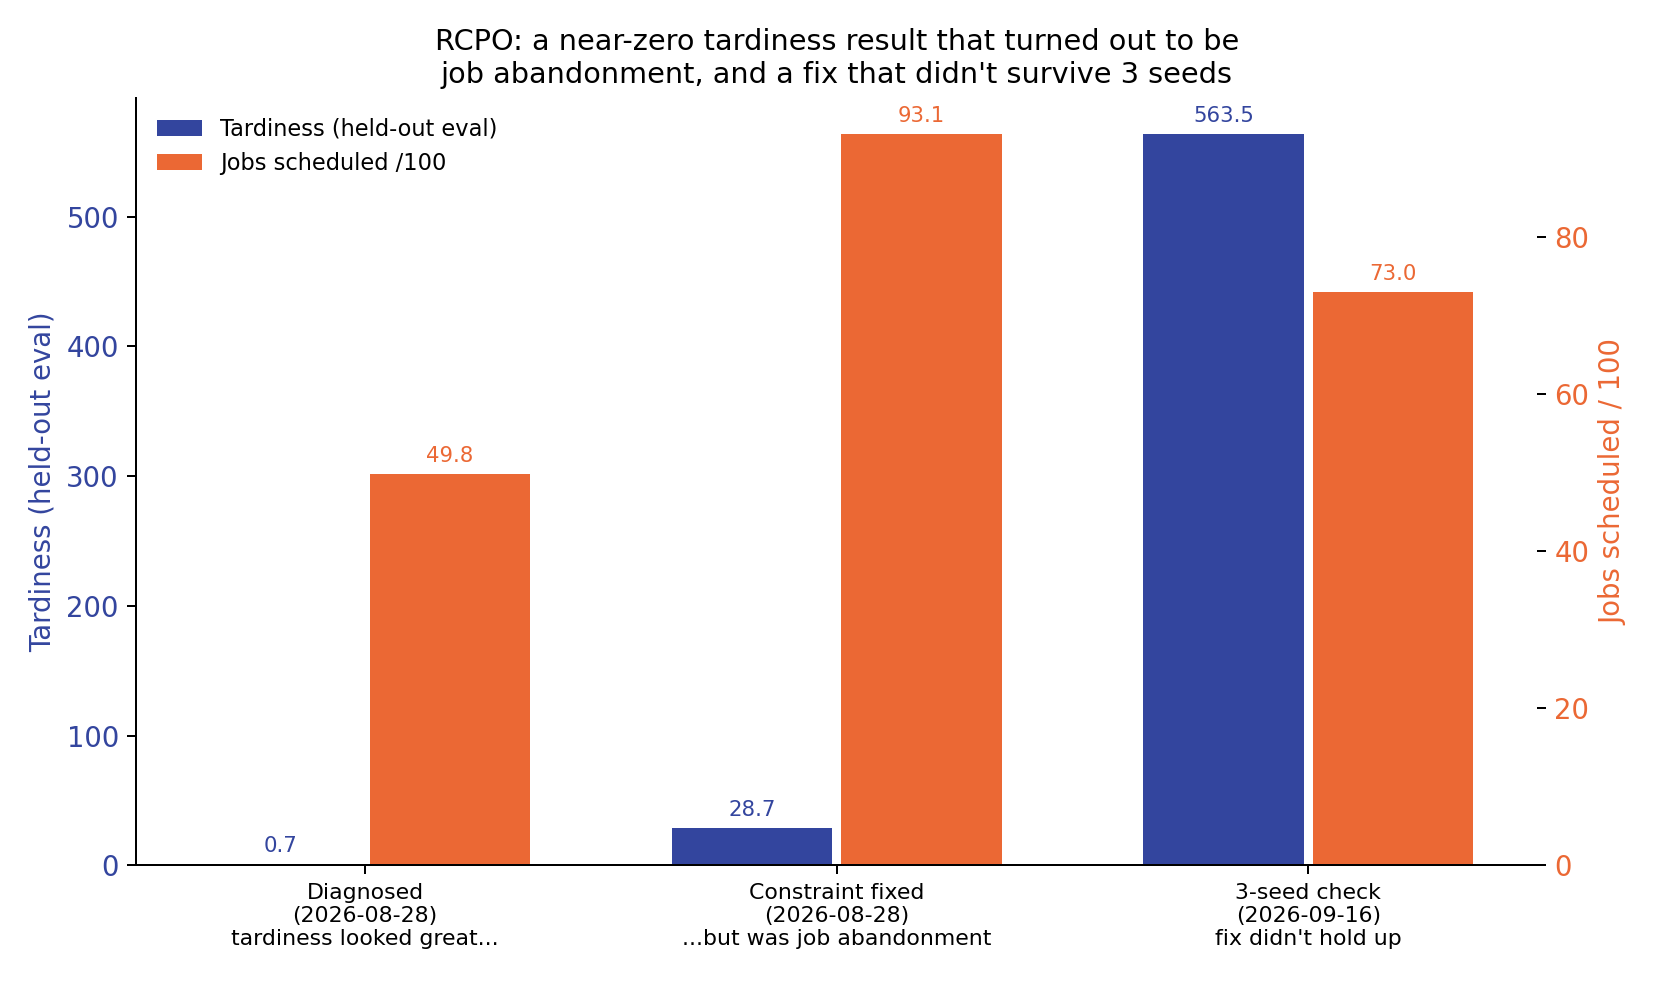
\includegraphics[width=0.85\textwidth]{../portfolio-artefacts/figures/rcpo_timeline.png}
\caption{RCPO: a near-zero tardiness result that was diagnosed as job abandonment, and a subsequent fix that did not survive a 3-seed rigor check.}
\label{fig:rcpo}
\end{figure}

\subsection{Offline Case: action-space reduction (Options 1--4)}
Reducing the action space, rather than further reward or hyperparameter tuning, was the change that resolved PPO's failure. Table~\ref{tab:action-space} shows the first-pass comparison (300k timesteps, un-tuned defaults, fixed instance): every option dramatically beats the historic PPO band, and the ranking matches the smaller/more-structured-action-space hypothesis exactly (Option 1's $\text{Discrete}(8) <$ Option 3's $\sim\text{Discrete}(101)$+ATC feature $<$ Option 2's plain $\sim\text{Discrete}(101)$).

\begin{table}[H]
\centering
\caption{Offline case, single fixed instance (100 jobs / 10 machines / horizon 100).}
\label{tab:action-space}
\begin{tabular}{lc}
\toprule
Method & Tardiness \\
\midrule
CP-SAT (proven optimal) & 8.00 \\
LST & 8.00 \\
Option 1, 1.2M timesteps, dense reward + real job weights & \textbf{11.00} \\
EDF & 16.00 \\
Option 1, 600k timesteps & 19.00 \\
Option 1, 300k timesteps & 35.00 \\
ATC & 106.00 \\
Option 3 (ATC-primed priority scoring) & 152.00 \\
Option 2 (raw-feature priority scoring) & 525.00 \\
Historic PPO (raw action space, best of 7 fixes tried) & $\sim$1290--1330 \\
\bottomrule
\end{tabular}
\end{table}

Doubling Option 1's training from 300k to 600k timesteps roughly halved its tardiness with no sign of plateauing; a later full-scale run (1.2M timesteps) combining action-space reduction with a per-tick dense reward and real (non-uniform) job weights reached 11.00 -- three units off the proven optimum, and ahead of every heuristic except LST (Figure~\ref{fig:offline-comparison}). Figure~\ref{fig:offline-comparison} shows the same result on a log scale, since the historic PPO band is more than two orders of magnitude worse than the best result -- the two cannot be shown clearly on a linear scale.

\begin{figure}[H]
\centering
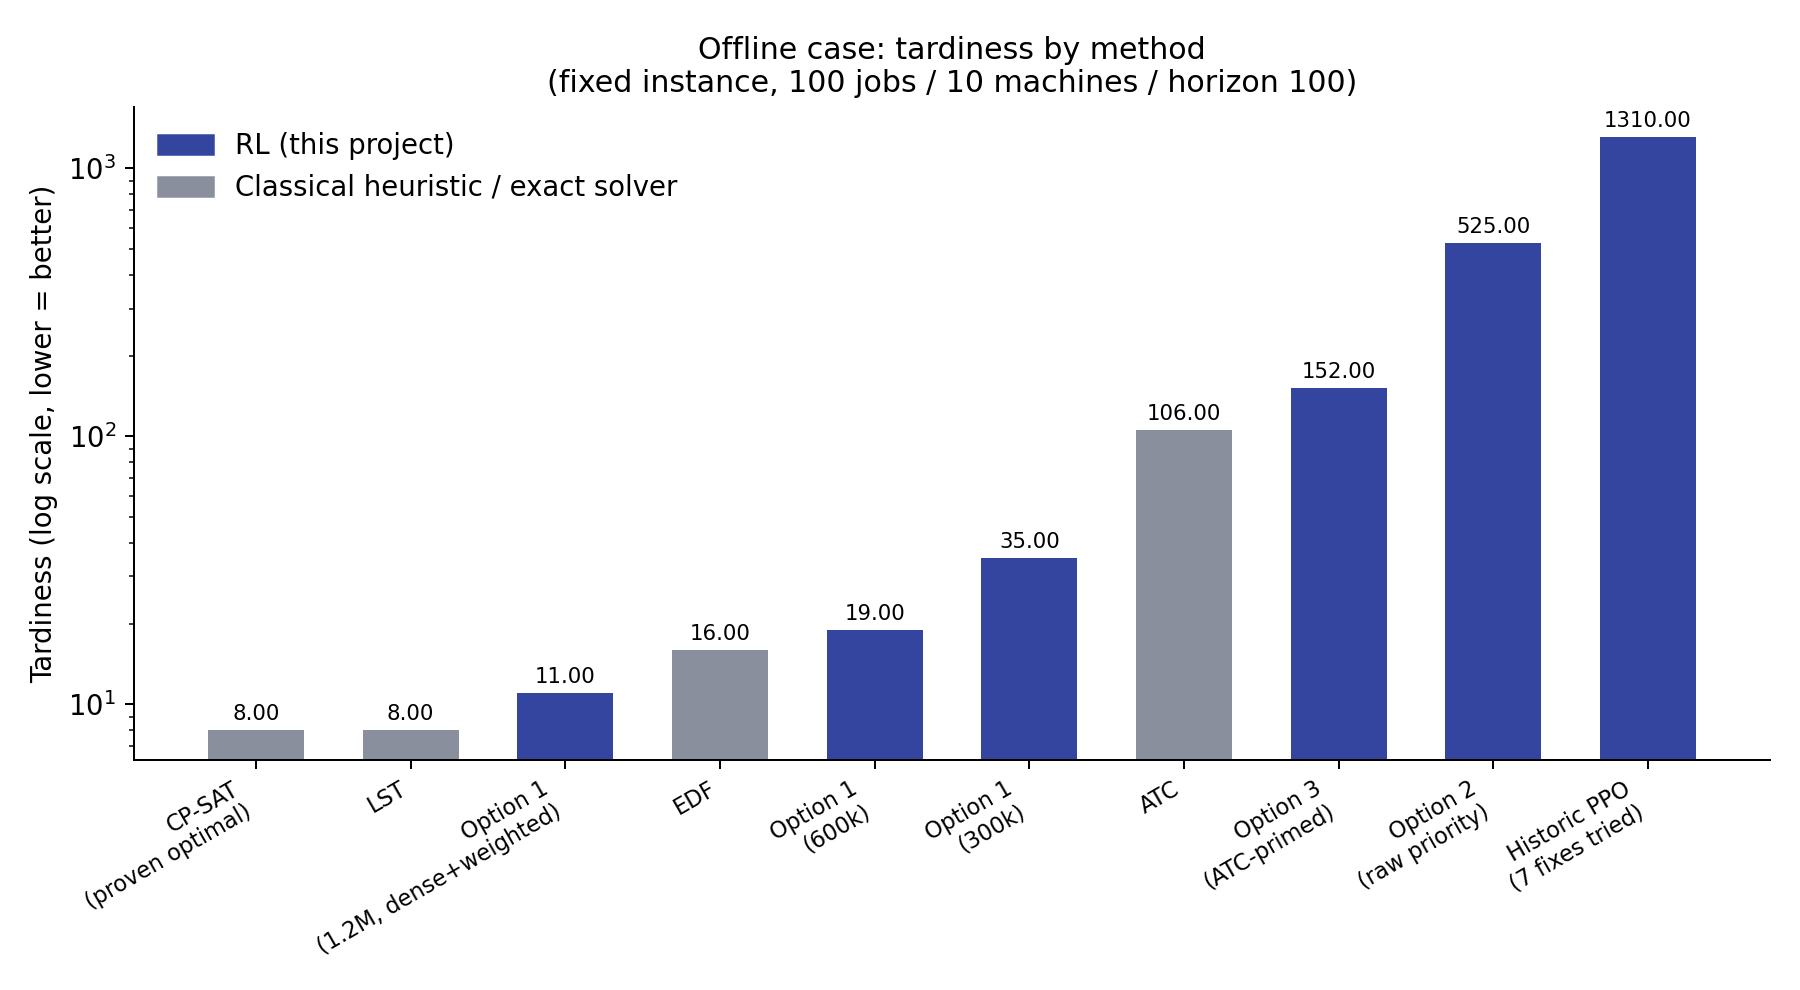
\includegraphics[width=0.95\textwidth]{../portfolio-artefacts/figures/offline_tardiness_comparison.png}
\caption{Offline case, every method compared on one log-scale chart.}
\label{fig:offline-comparison}
\end{figure}

This result requires a precise framing. Option 1's action space is literally "pick one of seven pre-written classical rules" -- it can never invent a genuinely new priority function, only learn \emph{when to defer} to an existing one. In the taxonomy of Burke et al. \cite{burke2013hyperheuristicsurvey}, this makes Option 1 a \emph{selection} hyper-heuristic, not a \emph{generation} one. The honest claim is therefore "an RL-trained hyper-heuristic that adaptively switches between classical rules beats any single fixed rule" -- a real, citable, literature-grounded result -- rather than "RL discovered novel scheduling behaviour," which would require Options 2 or 3 (which learn a priority function from raw features directly) to be the stronger result. They are currently weaker (152.00 and 525.00 respectively at first-pass scale), making genuinely novel-strategy-capable RL scheduling the actual open research direction here, not something this project has yet demonstrated.

On the randomized-instance distribution, the full-scale Option 1 (1.2M, dense reward + weights) reached tardiness 38.88 (weighted 116.50), an almost-exact tie with EDF (37.30 / 109.36) but still behind LST (23.94 / 68.62) -- action-space reduction closes most, but not all, of the generalisation gap that the earlier A2C result could not close at all.

Option 4 (action-branching, restoring a learned placement decision) was tested specifically to isolate whether Options 1--3's win came from the smaller action space or from skipping placement-learning entirely. At matched 300k-timestep budget, Option 4 (172.74 raw tardiness) was \emph{worse} than both Option 1 (49.32) and Option 3 (98.82) under the same dense-reward-plus-weights configuration -- direct evidence against the "it's really about not learning placement" explanation, and in favour of action-space size being the genuine driver. Three separate architectural refinements to Option 4's machine-placement pooling mechanism each unlocked a better achievable optimum during training (in one case reaching a perfect weighted tardiness of 0 mid-run) but were unable to reach that optimum reliably by the end of a fixed training budget -- an unresolved stability/optimum trade-off, not evidence that learned placement cannot work, only that it has not yet been made to work reliably here.

\subsection{Online Case}
\label{sec:online-results}
In the online setting, jobs arrive dynamically according to a Poisson process (full formulation in Section~\ref{sec:online} and the project's supporting research document). Under sustained heavy load, Options 1 and 3 (the two online-capable designs tested) outperform most classical heuristics, but neither has yet closed the gap to the strongest heuristic tested (ATC), and -- unlike the offline case, where more training reliably helped -- online training exhibits a robust, repeated regression with more timesteps (Figure~\ref{fig:online}). Option 1's best online result (weighted tardiness 730.30) was found at 300k timesteps; three independent runs at 900k timesteps (including one built specifically to defend against low-entropy premature convergence) all regressed to approximately 790--800, in one case becoming numerically \emph{identical, digit for digit}, to the SPT heuristic. This is not a single anomalous run: it has now been confirmed three times, across two different action-space designs (Option 1 and Option 3), ruling out noise or one bad seed as the explanation.

\begin{figure}[H]
\centering
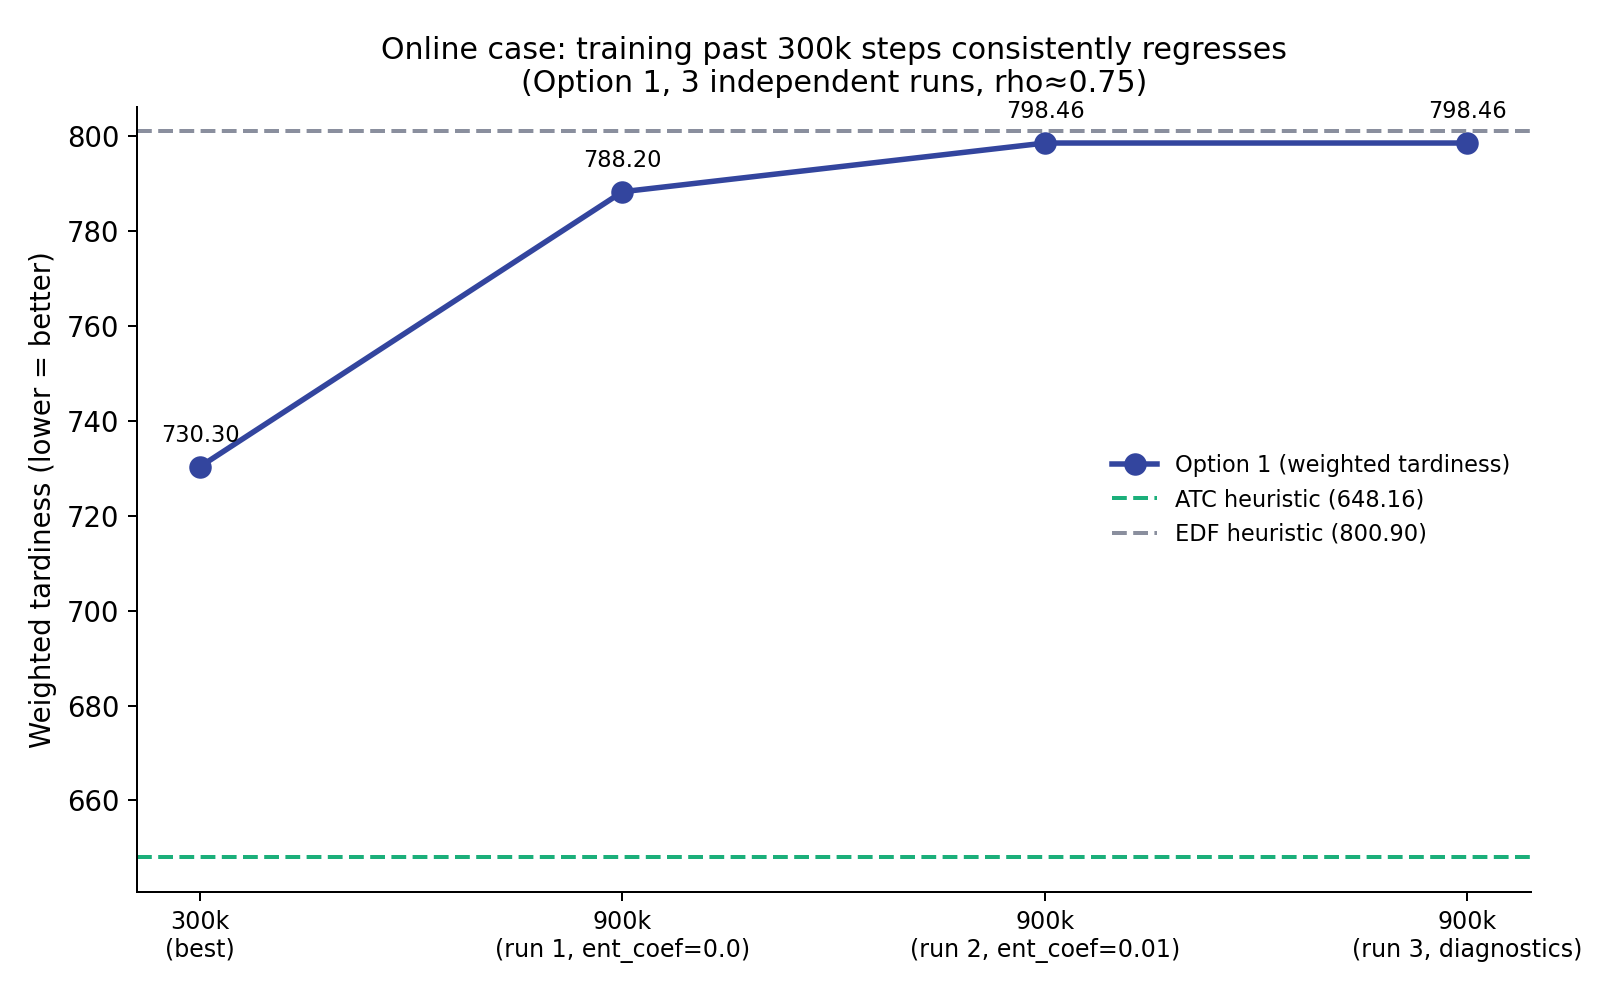
\includegraphics[width=0.85\textwidth]{../portfolio-artefacts/figures/online_more_training_hurts.png}
\caption{Online case: more training consistently regresses Option 1's performance, confirmed across three independent runs.}
\label{fig:online}
\end{figure}

A partial, literature-grounded explanation exists for \emph{why} the collapse converges specifically toward SPT rather than an arbitrary rule: SPT is the provably flow-time-optimal single-machine sequencing rule \cite{smith1956wspt}, and by Little's Law, minimising mean flow time also minimises mean waiting time under a fixed arrival rate -- a real, if partial, mechanism by which "clear the queue as fast as possible" is a locally attractive strategy under sustained heavy load, even though it ignores deadlines and weights entirely. This does not explain why the deterministic policy locks in and plateaus before the training-time entropy metric finishes decaying, nor why additional training pushes toward this local optimum rather than past it toward a weight-aware refinement (WSPT or ATC, both of which meaningfully outperform plain SPT under the same load conditions). Entropy regularisation was tested directly as a candidate fix and ruled out: training-time entropy stayed healthy throughout, but the deterministic policy still collapsed onto SPT, showing the earlier "zero entropy regularisation" diagnosis was incomplete. This remains the project's most significant open finding.

\section{Discussion}
This project set out to test, rather than assume, whether reinforcement learning can outperform traditional methods for cloud resource allocation -- and the honest answer is conditional. On the raw joint action space this project began with, RL (specifically PPO) categorically failed, across every literature-grounded fix attempted, to learn anything better than ignoring deadlines. That negative result is itself a genuine contribution: seven independent, well-motivated mechanisms (reward weighting, four Lagrangian ceiling variants, a tardiness-focused hyperparameter search, and a pointer-network architecture) were tried and ruled out before the actual driver -- action-space size -- was correctly identified by direct comparison against DeepRM and Decima's much smaller action spaces, and then confirmed by a clean single-variable ablation (Option 4) showing the improvement was not merely an artefact of no longer learning machine placement.

Once the action space was reduced, RL did outperform every classical heuristic tested except LST on the offline case, reaching within three tardiness units of a proven optimum. The relevance of this result is best stated precisely: it demonstrates that RL is an effective mechanism for \emph{learning when to apply which classical heuristic}, a genuinely useful and deployable capability (a hyper-heuristic selector needs no redesign to add a new rule to its repertoire, and adapts its rule choice to instance-specific conditions that a single fixed rule cannot). It does not yet demonstrate that RL can discover better scheduling policies than the best available classical rule from first principles -- the two designs capable of that (Options 2 and 3) are currently the weaker results, and closing that gap is the more ambitious, currently-unmet aim of the original project deliverables. The online case is less settled again: RL is competitive under load, but the discovery that additional training reliably makes it worse, converging toward a theoretically-explicable but deadline-blind rule, is a genuinely novel empirical finding for this specific environment, not just a gap in the results. Reporting it as an open, partially-understood phenomenon -- rather than omitting it or presenting only the best checkpoint found -- is, in the authors' view, more valuable to a reader than a cleaner but less honest story would be.

A second theme running through the results is the recurring gap between an initial positive result and what a more rigorous re-examination later found: RCPO's "best-ever" result was reward hacking; the earlier A2C win did not survive randomized-instance training; more online training looked like it should help and instead consistently hurt. None of these were caught by the first evaluation run that produced them -- each required either a follow-up instrumented diagnostic, a multi-seed rigor pass, or an independent repeat run to surface. This is presented not as a weakness of the project but as the central methodological lesson it produced: a single positive number, however striking, is not evidence until it has been stress-tested the way every result in this report eventually was.

\section{Conclusion}
Reinforcement learning did not outperform traditional scheduling heuristics in this project's original, most general formulation -- PPO on the raw job-and-machine action space failed unconditionally, and no amount of reward or hyperparameter tuning fixed it. When the action space was restructured around the insight that RL is well suited to \emph{selecting among} good policies rather than inventing one from an intractably large space of raw choices, the resulting hyper-heuristic came within three tardiness units of a proven-optimal solution and beat every classical heuristic tried except one. This is a genuine, literature-grounded, and honestly-scoped positive result, but a more modest one than the project's original framing ("can RL outperform traditional methods") implies at face value: the strongest evidence found is that RL outperforms any \emph{single} traditional method by learning to combine several of them, not that RL discovers scheduling behaviour beyond what the traditional literature already knows. The online case remains open, with a real, repeatedly-confirmed, and only partially-understood instability as its headline finding rather than a settled result either way.

\section{Future Work}
\begin{itemize}
    \item More research and consideration into the online case, including resolving the "more training hurts" instability before extending any further mechanism to it -- the online case remains incredibly complex and this project only touches on it.
    \item Look more into hybrid architectures \cite{ml_ra_litrev2025}, particularly generation hyper-heuristics (e.g. genetic programming evolving a pool of novel priority rules for Option 1's selection mechanism to choose among, rather than the seven hand-picked rules used here) \cite{chen2024drlgphh, xu2025learntooptimise}.
    \item Adopt simulation-based training and interactive learning environments \cite{ml_ra_litrev2025}.
    \item Consider more and different metrics and objectives, including an explicit, literature-grounded energy-efficiency term -- this project's existing hotspot penalty was found to actively work against, not for, the consolidation-based notion of energy efficiency in the literature \cite{fan2007powerprovisioning, energyaware2012}, and this tension is currently unresolved.
    \item Examine the large-action-space failure of policy-based methods further: replace the pointer-network job/machine encoding with graph neural networks \cite{gnn2024jsspsurvey}, and explore a wider range of action-space reductions and branching designs \cite{tavakoli2018actionbranching}.
    \item Evaluate large-discrete-action-space methods such as the Wolpertinger architecture \cite{dulacarnold2015largeactionspaces}.
    \item Investigate multi-agent formulations (e.g. MAPPO \cite{yu2022mappo}, QMIX \cite{rashid2018qmix}), which shrink the action space per machine-agent rather than requiring one policy to reason over the full joint space -- a structurally motivated extension of this project's own action-space-reduction findings.
    \item Isolate the algorithm effect between PPO and A2C directly: every "A2C beats PPO" result in this project is confounded by implementation (a hand-rolled A2C vs. a library PPO) and training infrastructure (vectorised vs. not) -- training a library A2C on the identical protocol used for PPO would settle this cleanly.
    \item Run a deployed-scale hyperparameter search specifically for Options 1--4, none of which have yet been tuned beyond un-tuned library defaults.
    \item Evaluate the trained policies against real-world cloud workload traces (e.g. the Google cluster trace or Microsoft Azure trace).
    \item Consider linked/dependent tasks (e.g. one job blocking another), an infinite (rather than fixed) planning horizon, and continuous-time decisions rather than integer ticks.
\end{itemize}

\section{Data Management Plan}
All code, experiment configuration, and the full chronological experiment log for this project are version-controlled and publicly available in this project's GitHub repository: \url{https://github.com/Ethan-Ty-Riekert/Neural-Knapsack-Research-Project}. Raw and processed evaluation results are stored as CSV files under \texttt{rl\_training/results/} (auto-appended by every evaluation run via \texttt{Code/utils/results\_log.py}) and are regenerable directly from the checked-in code and environment configuration rather than being the sole record of any result -- every number reported in this report traces back to a dated entry in \texttt{Future/research/training-log.md}, which records the exact configuration used to produce it. Trained model checkpoints and generated plots are build artefacts (regenerable from the code and are not committed to version control, consistent with standard practice for large binary outputs) but archived copies of key checkpoints referenced in this report are retained locally. The literature review and bibliography (\texttt{Future/research/references.bib}) are version-controlled alongside the code, with every entry's relevance documented in-line.

\section{GenAI Use Statement}
Generative AI (Claude, Anthropic) was used throughout this project in the following ways: (1) as a coding assistant for implementing the environment, RL policies, training/evaluation pipelines, and diagnostic tooling described in this report, under direct supervision and with all design decisions and their literature grounding directed or reviewed by the author; (2) to assist literature search and citation verification for the background research and design decisions summarised in this report; (3) to help diagnose unexpected experimental results (e.g. the RCPO reward-hacking finding in Section~\ref{sec:results} was surfaced through an AI-assisted instrumented re-evaluation, prompted by the author's request to investigate further, not discovered by the author manually); and (4) to assist in drafting and structuring this report from the author's own notes, data, and experiment log, with the author reviewing and editing the resulting text. No results, figures, or claims in this report were generated without the underlying code being run and its output directly inspected; generative AI was not used as a substitute for running experiments or verifying their results.

\newpage
%\nocite{*}
\bibliographystyle{IEEEtran}
\bibliography{../../Future/research/references}

\end{document}
